\chapter{Testing Hardy-Weinberg}

Because the Hardy-Weinberg principle tells us what to expect
concerning the genetic composition of a sample when no evolutionary
forces are operating, one of the first questions population
geneticists often ask is ``Are the genotypes in this sample present in
the expected, i.e., Hardy-Weinberg, proportions?'' We ask that
question because we know that if the genotypes are {\it not\/} in
Hardy-Weinberg proportions, at least one of the assumptions underlying
derivation of the principle has been violated, i.e., that there is
some evolutionary force operating on the population, and we know that
we can use the magnitude and direction of the departure to say
something about what those forces might be.

Of course we also know that the numbers in our sample may differ from
expectation just because of random sampling error. For example,
Table~\ref{table:MN-data} presents data from a sample of 1000 English
blood donors scored for MN phenotype. M and N are co-dominant, so that
heterozygotes can be distinguished from the two homozygotes. Clearly
the observed and expected numbers don't look very different. The
differences semm likely to be attributable purely to chance, but we
need some way of assessing that ``likeliness.''\index{testing Hardy-Weinberg}

\begin{table}
\begin{center}
\begin{tabular}{cccc}
\hline\hline
          &          & Observed & Expected \\
Phenotype & Genotype & Number   & Number   \\
\hline
M         & mm       & 298      & 294.3 \\
MN        & mn       & 489      & 496.3 \\
N         & nn       & 213      & 209.3 \\
\hline
\end{tabular}
\end{center}
\caption{Adapted from Table 2.4 in~\cite{Hedrick-2000}
  (from~\cite{Cleghorn-1960})}\label{table:MN-data} 
\end{table}

\section*{Testing Hardy-Weinberg}

One approach to testing the hypothesis that genotypes are in
Hardy-Weinberg proportions is quite simple. We can simply do a
$\chi^2$ or $G$-test for goodness of fit between observed and
predicted genotype (or phenotype) frequencies, where the predicted
genotype frequencies are derived from our estimates of the allele
frequencies in the population.\footnote{If you're not familiar with
  the $\chi^2$ or $G$-test for goodness of fit, consult any
  introductory statistics or biostatistics book, and you'll find a
  description. In fact, you probably don't have to go that far. You
  can probably find one in your old genetics textbook. Or you can just
  boot up your browser and head to Wikipedia:
  \myurl{http://en.wikipedia.org/wiki/Goodness\_of\_fit}. }\index{testing Hardy-Weinberg!goodness of fit} There's only one problem. To do
either of these tests we have to know how many degrees of freedom are
associated with the test. How do we figure that out? In general, the
formula is
\begin{eqnarray*}
\hbox{d.f.} = && (\hbox{\# of categories in the data -1 }) \\ 
&-& (\hbox{\#
              number of parameters estimated from the data})
\end{eqnarray*}
For this problem we have
\begin{eqnarray*}
\hbox{d.f.} = && (\hbox{\# of phenotype categories in the data - 1}) \\
&-& (\hbox{\# of allele frequencies estimated from the data})
\end{eqnarray*}
In the ABO blood group we have 4 phenotype categories, and 3
allele frequencies. That means that a test of whether a particular
data set has genotypes in Hardy-Weinberg proportions will have
$(4-1)-(3-1) = 1$ degrees of freedom for the test. Notice that this
also means that if you have completely dominant markers, like RAPDs or
AFLPs, you can't determine whether genotypes are in Hardy-Weinberg
proportions because you have 0 degrees of freedom available for the
test.

\subsection*{An example}

Table~\ref{table:abo-data} exhibits data drawn from a study of
phenotypic variation among individuals at the ABO blood locus:

\begin{table}
\begin{center}
\begin{tabular}{lccccc}
Phenotype &   A &  AB &   B &   O & Total \\
Observed  & 862 & 131 & 365 & 702 & 2060
\end{tabular}
\end{center}
\caption{Data on variation in ABO blood type.}\label{table:abo-data}
\end{table}
The maximum-likelihood estimate of allele frequencies,
assuming Hardy-Weinberg, is:\footnote{Take my word for it, or run the
  EM algorithm on these data yourself.}
\begin{eqnarray*}
p_a &=& 0.281 \\
p_b &=& 0.129 \\
p_o &=& 0.590 \quad , \\
\end{eqnarray*}
giving expected numbers of 846, 150, 348, and 716 for the
four phenotypes. $\chi^2_1 = 3.8$, $0.05 < p < 0.1$.

\section*{A Bayesian approach}

We saw last time how to use WinBUGS to provide allele frequency
estimates from phenotypic data at the \htmladdnormallink{ABO
  locus}{http://darwin.eeb.uconn.edu/eeb348/supplements-2004/multinomial-winbugs.txt}.\index{testing Hardy-Weinberg!Bayesian approach}
\begin{verbatim}
model {
   # likelihood 
   pi[1] <- p.a*p.a + 2*p.a*p.o
   pi[2] <- 2*p.a*p.b
   pi[3] <- p.b*p.b + 2*p.b*p.o
   pi[4] <- p.o*p.o
   x[1:4] ~ dmulti(pi[],n)

   # priors
   a1 ~ dexp(1)
   b1 ~ dexp(1)
   o1 ~ dexp(1)
   p.a <- a1/(a1 + b1 + o1)
   p.b <- b1/(a1 + b1 + o1)
   p.o <- o1/(a1 + b1 + o1)

   n <- sum(x[])
}

list(x=c(862, 131, 365, 702))
\end{verbatim}
As you may recall, this produced the results in
Figure~\ref{fig:multinomial-results}.

\begin{figure}
\resizebox{\textwidth}{!}{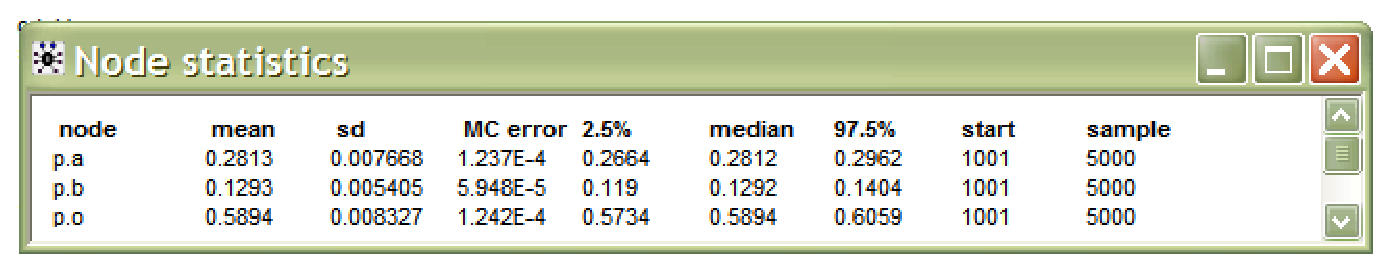
\includegraphics{multinomial-results.eps}}
\caption{Results from WinBUGS analysis of the ABO
  data assuming genotypes are in Hardy-Weinberg proportions.}\label{fig:multinomial-results}
\end{figure}

Now that we know about inbreeding coefficients and that the allow us
to measure the departure of genotype frequencies from Hardy-Weinberg
proportions, we can modify this a bit and estimate allele frequencies
without assuming that genotypes are in Hardy-Weinberg proportions.
\begin{verbatim}
model {
   # likelihood 
   pi[1] <- p.a*p.a + f*p.a*(1-p.a) + 2*p.a*p.o*(1-f)
   pi[2] <- 2*p.a*p.b*(1-f)
   pi[3] <- p.b*p.b + f*p.b*(1-p.b) + 2*p.b*p.o*(1-f)
   pi[4] <- p.o*p.o + f*p.o*(1-p.o)
   x[1:4] ~ dmulti(pi[],n)

   # priors
   a1 ~ dexp(1)
   b1 ~ dexp(1)
   o1 ~ dexp(1)
   p.a <- a1/(a1 + b1 + o1)
   p.b <- b1/(a1 + b1 + o1)
   p.o <- o1/(a1 + b1 + o1)

   f ~ dunif(0,1)

   n <- sum(x[])
}

list(x=c(862, 131, 365, 702))
\end{verbatim}
This produces the results in Figure~\ref{fig:ABO-inbreeding}

\begin{figure}
\resizebox{\textwidth}{!}{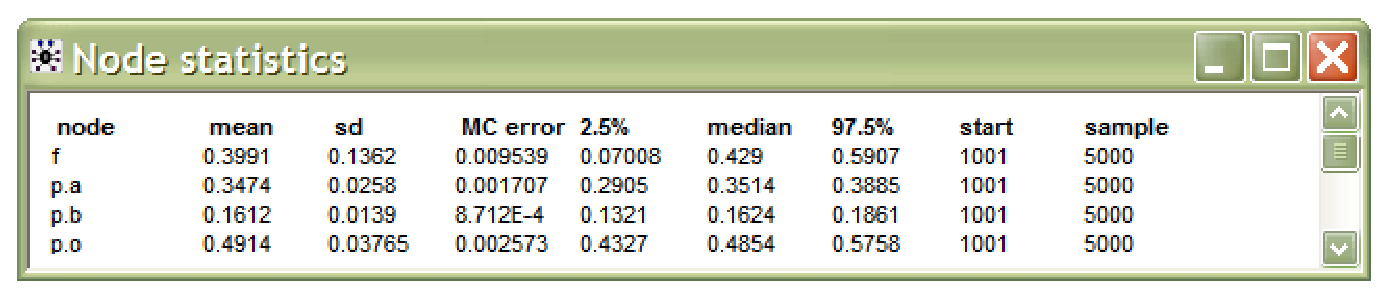
\includegraphics{ABO-inbreeding.eps}}
\caption{Results from WinBUGS analysis of the ABO
  data relaxing the assumption that genotypes are in Hardy-Weinberg proportions.}\label{fig:ABO-inbreeding}
\end{figure}

Notice that the allele frequency estimates have changed quite a bit
and that the posterior mean of $f$ is about 0.41. On first appearance,
that would seem to indicate that we have lots of inbreeding in this
sample. {\bf BUT} it's a human population. It doesn't seem very
likely that a human population is really that highly inbred. 

Indeed, take a closer look at {\it all\/} of the information we have
about that estimate of $f$. The 95\% credible interval for $f$ is
between 0.06 and 0.55. That suggests that we don't have much
information at all about $f$ from these data.\footnote{That shouldn't
  be too surprising, since any information we have about $f$ comes
  indirectly through our allele frequency estimates.} How can we tell
if the model with inbreeding is better than the model that assumes
genotypes are in Hardy-Weinberg proportions?

\subsection*{The Deviance Information Criterion}

A widely used statistic for comparing models in a Bayesian framework
is the Deviance Information Criterion.\index{Deviance Information Criterion} It can be calculated automatically in WinBUGS, just by
clicking the right button. The results of the DIC calculations for our
two models are summarized in Table~\ref{table:ABO-dic}.

\begin{table}
\begin{center}
\begin{tabular}{c|cccc}
\hline\hline
Model   & Dbar   & Dhat   & pD    & DIC \\
\hline
$f > 0$ & 24.900 & 22.319 & 2.581 & 24.480 \\
$f = 0$ & 27.827 & 25.786 & 2.041 & 29.869 \\
\hline
\end{tabular}
\end{center}
\caption{DIC calculations for the ABO example.}\label{table:ABO-dic}
\end{table}

Dbar and Dhat are measures of how well the model fits the data. Dbar
is the posterior mean log likelihood, i.e., the average of the log
likelihood values calculated from the parameters in each sample from
the posterior. Dhat is the log likelihood at the posterior mean, i.e.,
the log likelihood calcuated when all of the parameters are set to
their posterior mean. pD is a measure of model complexity, roughly
speaking the number of parameters in the model. DIC is a composite
measure of how well the model does. It's a compromise between fit and
complexity, and smaller DICs are preferred. A difference of more than
7-10 units is regarded as strong evidence in favor of the model with
the smaller DIC. 

In this case the difference in DIC values is about 5.5, so we have
some evidence for $f > 0$ model for these data, even though they are
from a human population. But the evidence is not very strong. This is
consistent with the weak evidence for a departure from Hardy-Weinberg
that was revealed in the $\chi^2$ analysis.

